\documentclass[a4paper,12pt]{jsbook}
\setlength{\textwidth}{\fullwidth}
\setlength{\evensidemargin}{\oddsidemargin}
\usepackage{thesis}
\usepackage{makeidx}
\usepackage{amsmath}
\usepackage{txfonts, float}
\usepackage{here}
\usepackage[dvipdfmx]{graphicx}
%\usepackage[noto-otc, unicode]{pxchfon}
\usepackage{subfiles}
\usepackage[backend=bibtex,style=phys,articletitle=true,biblabel=brackets,chaptertitle=false,pageranges=false]{biblatex}
\addbibresource{./bib/liter.bib}

\begin{document}

% 表紙
\thesis{修士論文}
\date{20xx年xx月xx日}
\title{
    \scalebox{1.5}{The Title}\\
    \vspace{1.2zh}
    \scalebox{1.5}{of}\\
    \vspace{1.2zh}
    \scalebox{1.5}{Your Master Thesis}
}
\teacher{Your Professor 教授}
\organization{名古屋大学大学院 理学研究科 物質理学専攻(物理系)}
\labname{your labname}
\author{Your Name}
\idnumber{Your ID}

\maketitle

% 前書き
\documentclass[../thesis.tex]{subfiles}
% このファイル内だけのコマンド
\begin{document}
\begin{center}
\Large{概要}
\end{center}
\normalsize
\thispagestyle{empty}
先行研究では、...ということが知られている。
\end{document}
\frontmatter
\tableofcontents

%画像の目次
%\listoffigures

%図の目次
%\listoftables

% 本文
\mainmatter
%\documentclass[../thesis]{subfiles}
% このファイル内だけのコマンド
\begin{document}
\chapter{How To Use \LaTeX}

\section{Figure}
    \subsection{基本的な画像挿入方法}
    写真はimg下に配置します.\\
    \begin{figure}[htbp]
        \centering   
        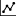
\includegraphics[width=0.5\textwidth]{img/sample/sample_png.png}
        \label{fig:sample_png}
        \caption[sample image (png)]{sample image: when its extension is png.}
    \end{figure}
    labelで指定することで, \figref{fig:sample_png}はxxxのように参照することができる.\\
    captionでは [] が目次に示される内容で, \{\} が本文に示される内容である. 同じでいい場合は \{\} のみで良い.\\
    上記のように, pngやjpegのようなラスタ画像を用いると, 拡大したときに荒くなってしまう.\\
    下記のようにpdfのようなベクタ画像を用いると拡大しても荒くならない.
    ただし, 保存時にベクタ形式にする必要がある.
    \begin{figure}[htbp]
        \centering   
        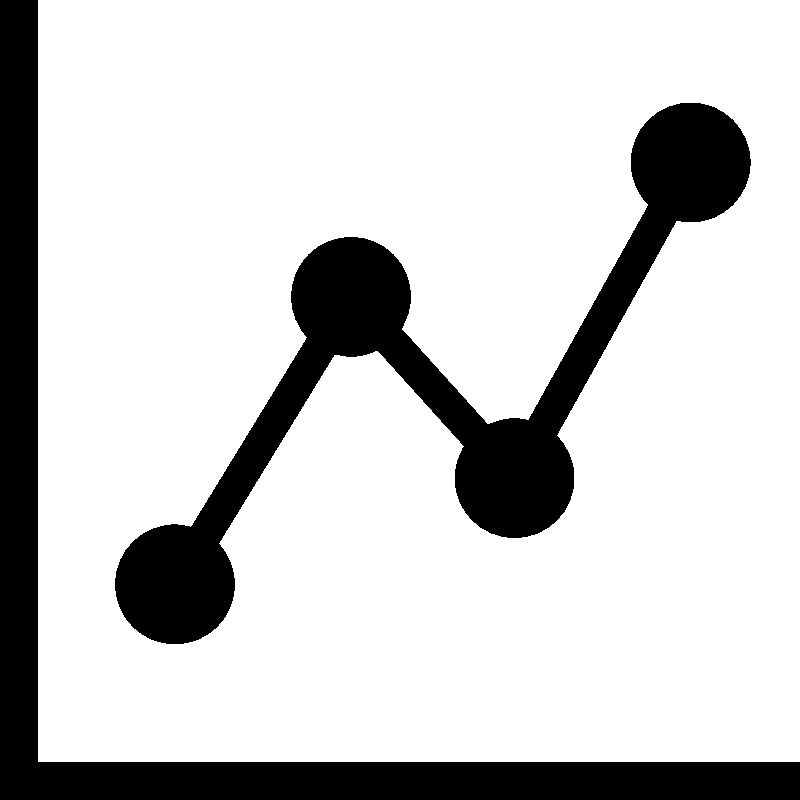
\includegraphics[width=0.5\textwidth]{img/sample/sample_pdf.pdf}
        \label{Fig:sample_pdf}
        \caption[sample image (pdf)]{sample image: when its extension is pdf.}
    \end{figure}
    出力の位置は[htbp]で指定するが, レイアウトによっては自動的に次のページに移動するなど, 指定した通りに配置できないときがある.\\
    この場合は[H]のように大文字で指定すると,
    \begin{figure}[H]
        \centering   
        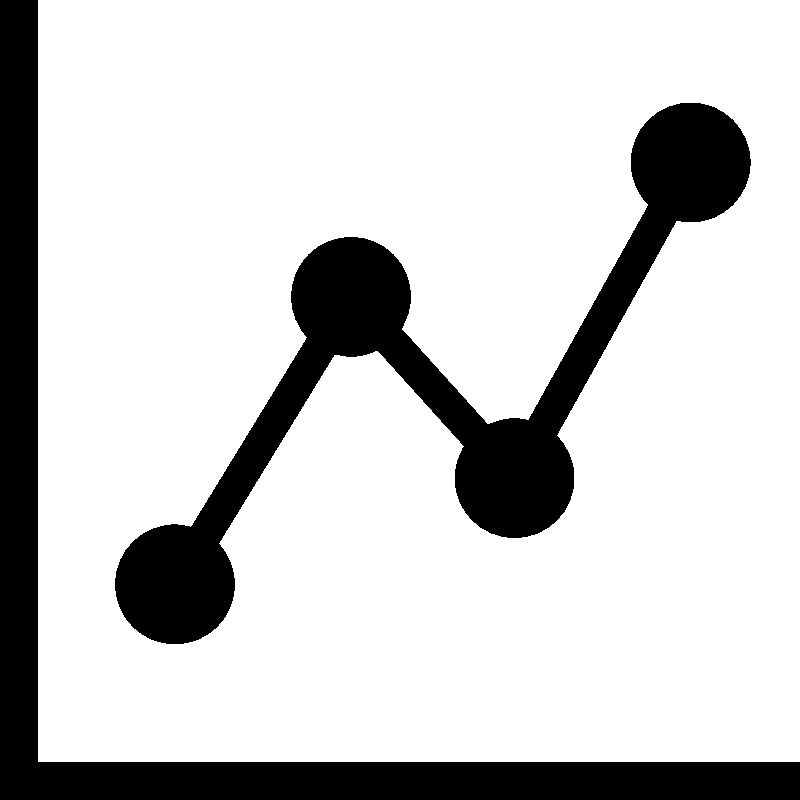
\includegraphics[width=0.5\textwidth]{img/sample/sample_pdf.pdf}
        \label{Fig:sample_pdf_here}
        \caption[sample image (pdf, here)]{sample image: when its extension is pdf and is enforced to be here.}
    \end{figure}
    このように強制的に配置が可能になる.

    \subsection{複数画像の挿入}
    複数画像の挿入方法はいくつかあるようだが, とりあえず下記で挿入することが可能.
    \begin{figure}[H]
		\centering
		\begin{tabular}{c}
		% ----- image 1 =====
			\begin{minipage}{0.25\hsize}
				\centering
				
\includegraphics[width=\textwidth]{img/sample/sample1.pdf}
				\text{(a)}
			\end{minipage}
		% ----- image 2 =====
			\begin{minipage}{0.25\hsize}
				\centering
				
\includegraphics[width=\textwidth]{img/sample/sample2.pdf}
				\text{(b)}
			\end{minipage}
		% ----- image 3 =====
			\begin{minipage}{0.25\hsize}
				\centering
				
\includegraphics[width=\textwidth]{img/sample/sample3.pdf}
				\text{(c)}
			\end{minipage}
		% ----- image 4 =====
			\begin{minipage}{0.25\hsize}
				\centering
				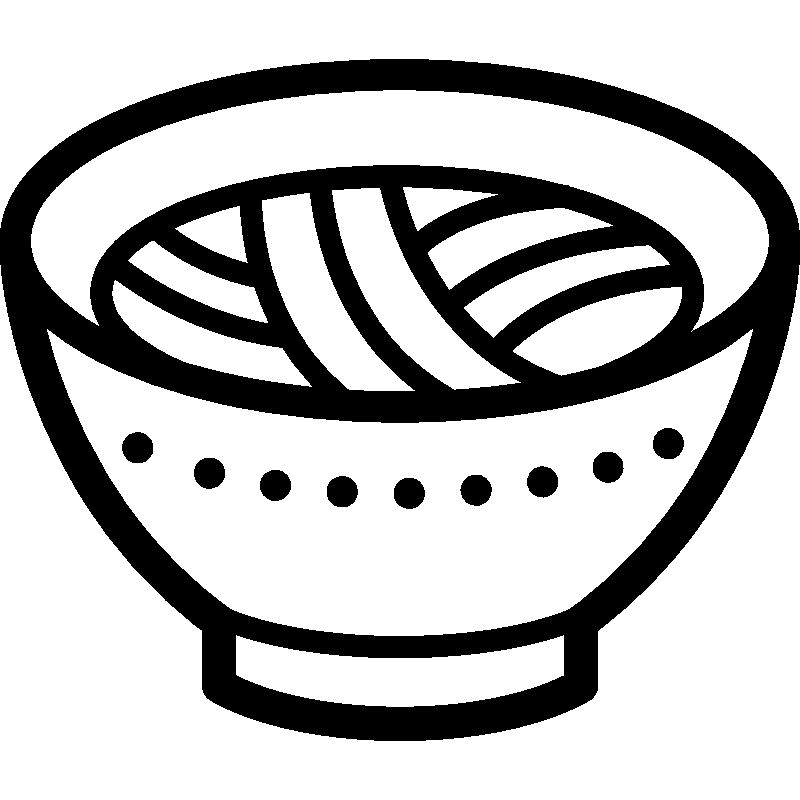
\includegraphics[width=\textwidth]{img/sample/sample4.pdf}
				\text{(d)}
			\end{minipage}
		\end{tabular}
		\caption[Four sample images]
		{
			Four sample images.
			(a) sushi (b) milk (c) peach (d) ramen
		}
		\label{fig:sample_four_images}
	\end{figure}

    縦2横2にすることも可能.
    \begin{figure}[H]
		\centering
		\begin{tabular}{c}
		% ----- image 1 =====
			\begin{minipage}{0.25\hsize}
				\centering
				
\includegraphics[width=\textwidth]{img/sample/sample1.pdf}
				\text{(a)}
			\end{minipage}
			\hspace{1cm}
		% ----- image 2 =====
			\begin{minipage}{0.25\hsize}
				\centering
				
\includegraphics[width=\textwidth]{img/sample/sample2.pdf}
				\text{(b)}
			\end{minipage}
			\vspace{1cm}\\
		% ----- image 3 =====
			\begin{minipage}{0.25\hsize}
				\centering
				
\includegraphics[width=\textwidth]{img/sample/sample3.pdf}
				\text{(c)}
			\end{minipage}
			\hspace{1cm}
		% ----- image 4 =====
			\begin{minipage}{0.25\hsize}
				\centering
				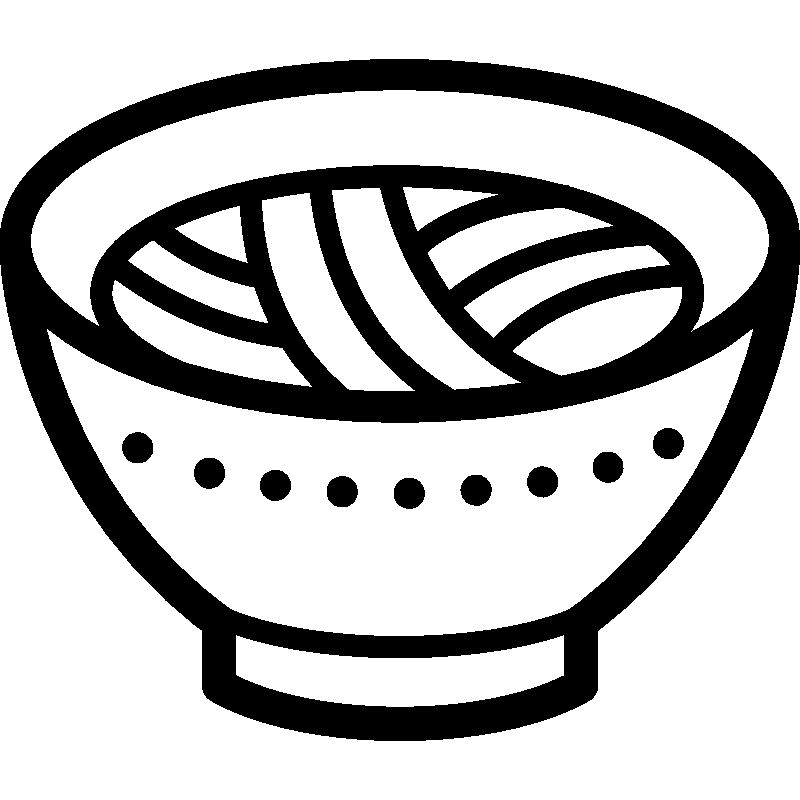
\includegraphics[width=\textwidth]{img/sample/sample4.pdf}
				\text{(d)}
			\end{minipage}
		\end{tabular}
		\caption[Four sample images]
		{
			Four sample images 2.
			(a) sushi (b) milk (c) peach (d) ramen
		}
		\label{fig:sample_four_images2}
	\end{figure}
    
\section{Table}
Tableは\tbref{tb:sample_table}のようにして挿入する.
\begin{table}[H]
	\centering
	\caption{Sample Table: accuracy for train/evaluation data.}
	\begin{tabular}{ll}\hline
		 訓練データの正答率&: $98\%$ \\
		 テストデータの正答率&: $88\%$ \\
	\label{tb:sample_table}
	\end{tabular}
\end{table}

\section{Bib}
参考文献は, \cite{author:06}とすれば良い.
複数の参考文献を扱う場合は, \cite{author:06, conference:06}のようにする.\\
使用してない参考文献は自動的に記載されないようになっているので, とりあえずbib/liter.bibに入れておいて構わない.\\
通し番号は本文で言及された順になるがこれも自動的に処理されるので気にしなくて良い.

\section{Equation}
数式の入力はたくさんある.
文章中であれば, $x = 2$ のように挿入できる.\\
数式環境を用意する場合は, \equref{eq:sample1}, \equref{eq:sample2}, \equref{eq:sample3}のようにできる.

\begin{align}
    x &= 2 \label{eq:sample1}\\
    y &= x^2 + 1 \label{eq:sample2}\\
      &= 5 \label{eq:sample3}
\end{align}
\end{document} % 使い方を示す例
\subfile{chapter/introduction}
\subfile{chapter/background}
\subfile{chapter/proposed}
\subfile{chapter/result}
\subfile{chapter/result2}
\subfile{chapter/conclusion}
\subfile{chapter/acknowledgement}
\subfile{chapter/bibliography}
\subfile{chapter/appendix1}
\subfile{chapter/appendix2}

% 後書き
\backmatter
\appendix

\printindex
\end{document}